\documentclass[tikz,border=7pt]{standalone}
\usepackage{amsmath}
\usetikzlibrary{positioning,arrows.meta}
\tikzset{box/.style={draw,rectangle,rounded corners=2pt,minimum width=64mm,minimum height=42mm,align=left},arr/.style={-{Latex[length=2mm]},thick}}
\begin{document}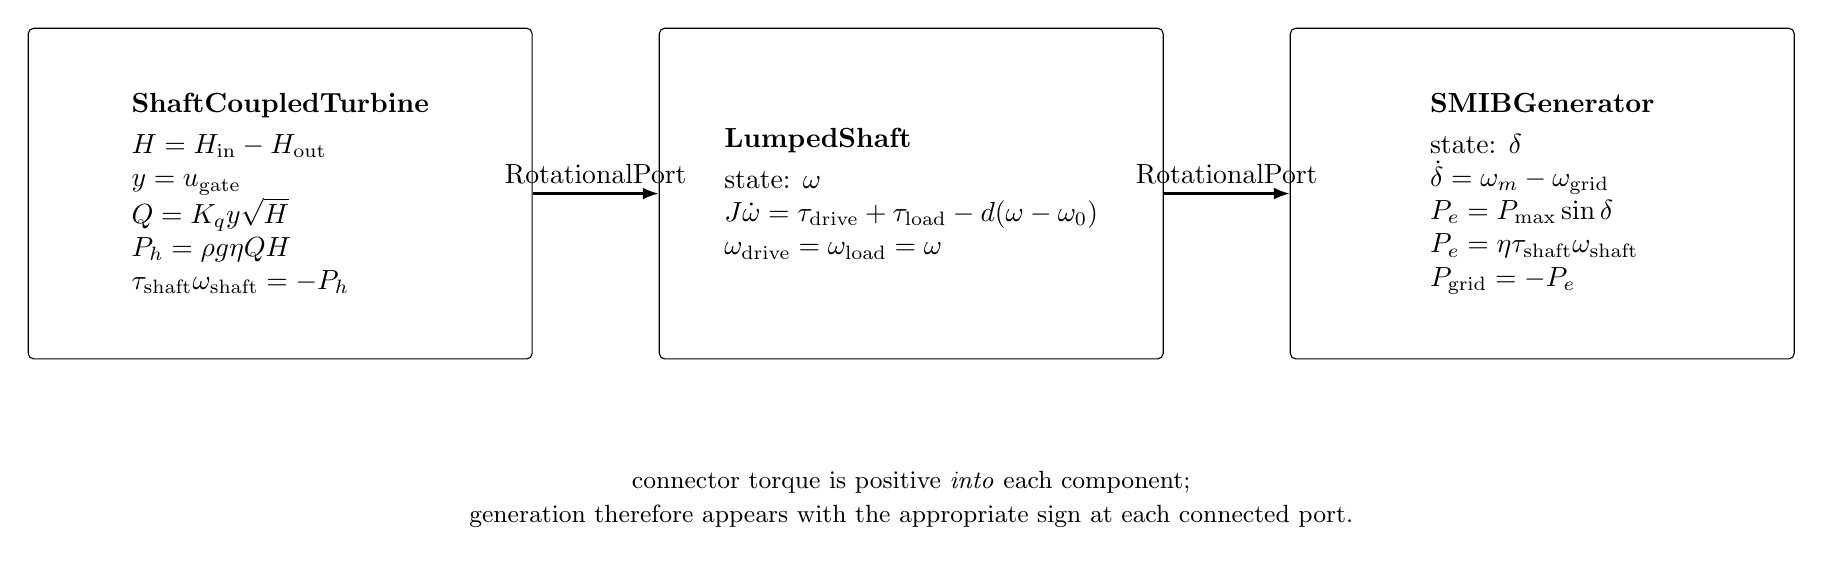
\begin{tikzpicture}[node distance=16mm]
\node[box] (turb) {\textbf{ShaftCoupledTurbine}\\[1mm]
$H=H_{\rm in}-H_{\rm out}$\\
$y=u_{\rm gate}$\\
$Q=K_q y\sqrt{H}$\\
$P_h=\rho g\eta QH$\\
$\tau_{\rm shaft}\omega_{\rm shaft}=-P_h$};
\node[box,right=of turb] (shaft) {\textbf{LumpedShaft}\\[1mm]
state: $\omega$\\
$\displaystyle J\dot\omega=\tau_{\rm drive}+\tau_{\rm load}-d(\omega-\omega_0)$\\
$\omega_{\rm drive}=\omega_{\rm load}=\omega$};
\node[box,right=of shaft] (gen) {\textbf{SMIBGenerator}\\[1mm]
state: $\delta$\\
$\dot\delta=\omega_m-\omega_{\rm grid}$\\
$P_e=P_{\max}\sin\delta$\\
$P_e=\eta\tau_{\rm shaft}\omega_{\rm shaft}$\\
$P_{\rm grid}=-P_e$};
\draw[arr] (turb) -- node[above] {RotationalPort} (shaft);
\draw[arr] (shaft) -- node[above] {RotationalPort} (gen);
\node[below=13mm of shaft,align=center] {\small connector torque is positive \emph{into} each component;\\
\small generation therefore appears with the appropriate sign at each connected port.};
\end{tikzpicture}\end{document}
